\documentclass[12pt]{beamer}

% \usepackage[sc]{mathpazo}
% \linespread{1.05}
\usepackage[T1]{fontenc}
\usepackage[francais]{babel}

\usepackage{lmodern}
%\usetheme{Szeged}
\usepackage{fontspec}
\usepackage{graphicx}

\usepackage{hyperref}
\usepackage{minted}
\usepackage{tikz}

% BEGIN STYLE

\setbeameroption{hide notes}
\setbeamertemplate{note page}[plain]

\usetheme{default}
\beamertemplatenavigationsymbolsempty
\hypersetup{pdfpagemode=UseNone}

\setmonofont{Inconsolata}

\usefonttheme{professionalfonts}
\usefonttheme{serif}
\usepackage{fontspec}
\setmainfont{Helvetica Neue}
\setbeamerfont{note page}{family*=pplx,size=\footnotesize}

\definecolor{latexblue}{RGB}{87,102,181}

\definecolor{foreground}{RGB}{21,21,21}
\definecolor{background}{RGB}{242,245,227}
\definecolor{title}{RGB}{27,130,63}
\definecolor{gray}{RGB}{155,155,155}
\definecolor{subtitle}{RGB}{102,255,204}
\definecolor{hilight}{RGB}{102,255,204}
\definecolor{vhilight}{RGB}{255,111,207}

\useinnertheme{rectangles}

\setbeamercolor{background canvas}{bg=background}
\setbeamercolor{titlelike}{fg=title}
\setbeamercolor{subtitle}{fg=subtitle}
\setbeamercolor{institute}{fg=gray}
\setbeamercolor{normal text}{fg=foreground,bg=background}
\setbeamercolor{item projected}{bg=foreground, fg=background}
\setbeamercolor{structure}{fg=foreground}
\setbeamercolor{subitem}{fg=foreground}
\setbeamercolor{itemize/enumerate subbody}{fg=foreground}

\setbeamertemplate{itemize subitem}{{\textendash}}

\setbeamerfont{itemize/enumerate subbody}{size=\footnotesize}
\setbeamerfont{itemize/enumerate subitem}{size=\footnotesize}

\setbeamertemplate{footline}{
    \raisebox{5pt}{\makebox[\paperwidth]{\hfill\makebox[20pt]{\color{gray}
\scriptsize\insertframenumber}}}\hspace*{5pt}}

\addtobeamertemplate{note page}{\setlength{\parskip}{12pt}}

\newminted{csharp}{bgcolor=gray!25,fontsize=\footnotesize,mathescape}

% END STYLE

\title[Bien démarrer son projet]{\textbf{Bien démarrer son projet}}

\author{
    Valentin 'toogy' Iovene \\
    Alexis 'Horgix' Chotard \\
    Théophile 'yroeht' Ranquet
}

\institute{
\includegraphics[scale=0.38]{img/logos.png}}

\date{}

\begin{document}

{
    \setbeamertemplate{footline}{} % no page number here
    \frame{
        \titlepage
    }
}

\section*{Introduction}

\begin{frame}
    \frametitle{La conférence}
    \tableofcontents[pausesections]
\end{frame}

\section{Organiser son projet et maintenir son code}

\begin{frame}
    \begin{center}
        \vspace{1cm}
        {\Large \textbf{1.} Organiser son projet\\
        et maintenir son code \\}
    \end{center}
\end{frame}

\begin{frame}
    \begin{center}
        \vspace{1cm}
        {\large Organiser son \textbf{projet}}
    \end{center}
\end{frame}

\begin{frame}[fragile]
    \begin{center}
        \vspace{1cm}
        {\large Réfléchir avant d'agir (de coder)} \\
    \end{center}
\end{frame}

\begin{frame}
    \vspace{1cm}
    {\large \textbf{Avoir les idées claires, savoir où on va}} \\
    \begin{itemize}
        \pause \item Brainstorming : trouver ce qu'on \textbf{veut} faire \\
        \pause \item Fixer un but \emph{concret} à atteindre (le produit)
        \pause \item Représenter son projet visuellement
    \end{itemize}
\end{frame}

\begin{frame}
    \vspace{1cm}
    {\large \textbf{Découper son projet en fonctionnalités}} \\
    \begin{itemize}
        \pause\item Menu \\
        \pause\item Minimap \\
        \pause\item Map \\
        \pause\item Unités \\
        \begin{itemize}
            \pause\item Ouvrier \\
            \begin{itemize}
                \pause\item Récolte \\
                \pause\item Construction de bâtiments \\
            \end{itemize}
            \pause\item Combats \\
            \pause\item Déplacements \\
        \end{itemize}
        \pause\item Système de ressources \\
        \pause\item Bâtiments \\
        \begin{itemize}
            \pause\item File d'attente de création d'unités \\
            \pause\item Point de ralliement \\
        \end{itemize}
    \end{itemize}
\end{frame}

\begin{frame}
    \vspace{1cm}
    {\large \textbf{Priorisation (valeur ajoutée + dépendance)}} \\
    \begin{itemize}
        \item Map \\
        \item Unités \\
        \item Unités:Déplacements \\
        \item Système de ressources \\
        \item Bâtiments \\
        \item Unités:Ouvrier:Récolte \\
        \item Unités:Ouvrier:Construction de bâtiments \\
        \item Unités:Combats \\
        \item Bâtiments:File d'attente de création d'unités \\
        \item Bâtiments:Point de ralliement \\
        \item Minimap \\
        \item Menu \\
    \end{itemize}
\end{frame}

{ % all template changes are local to this group.
    \setbeamertemplate{background canvas}{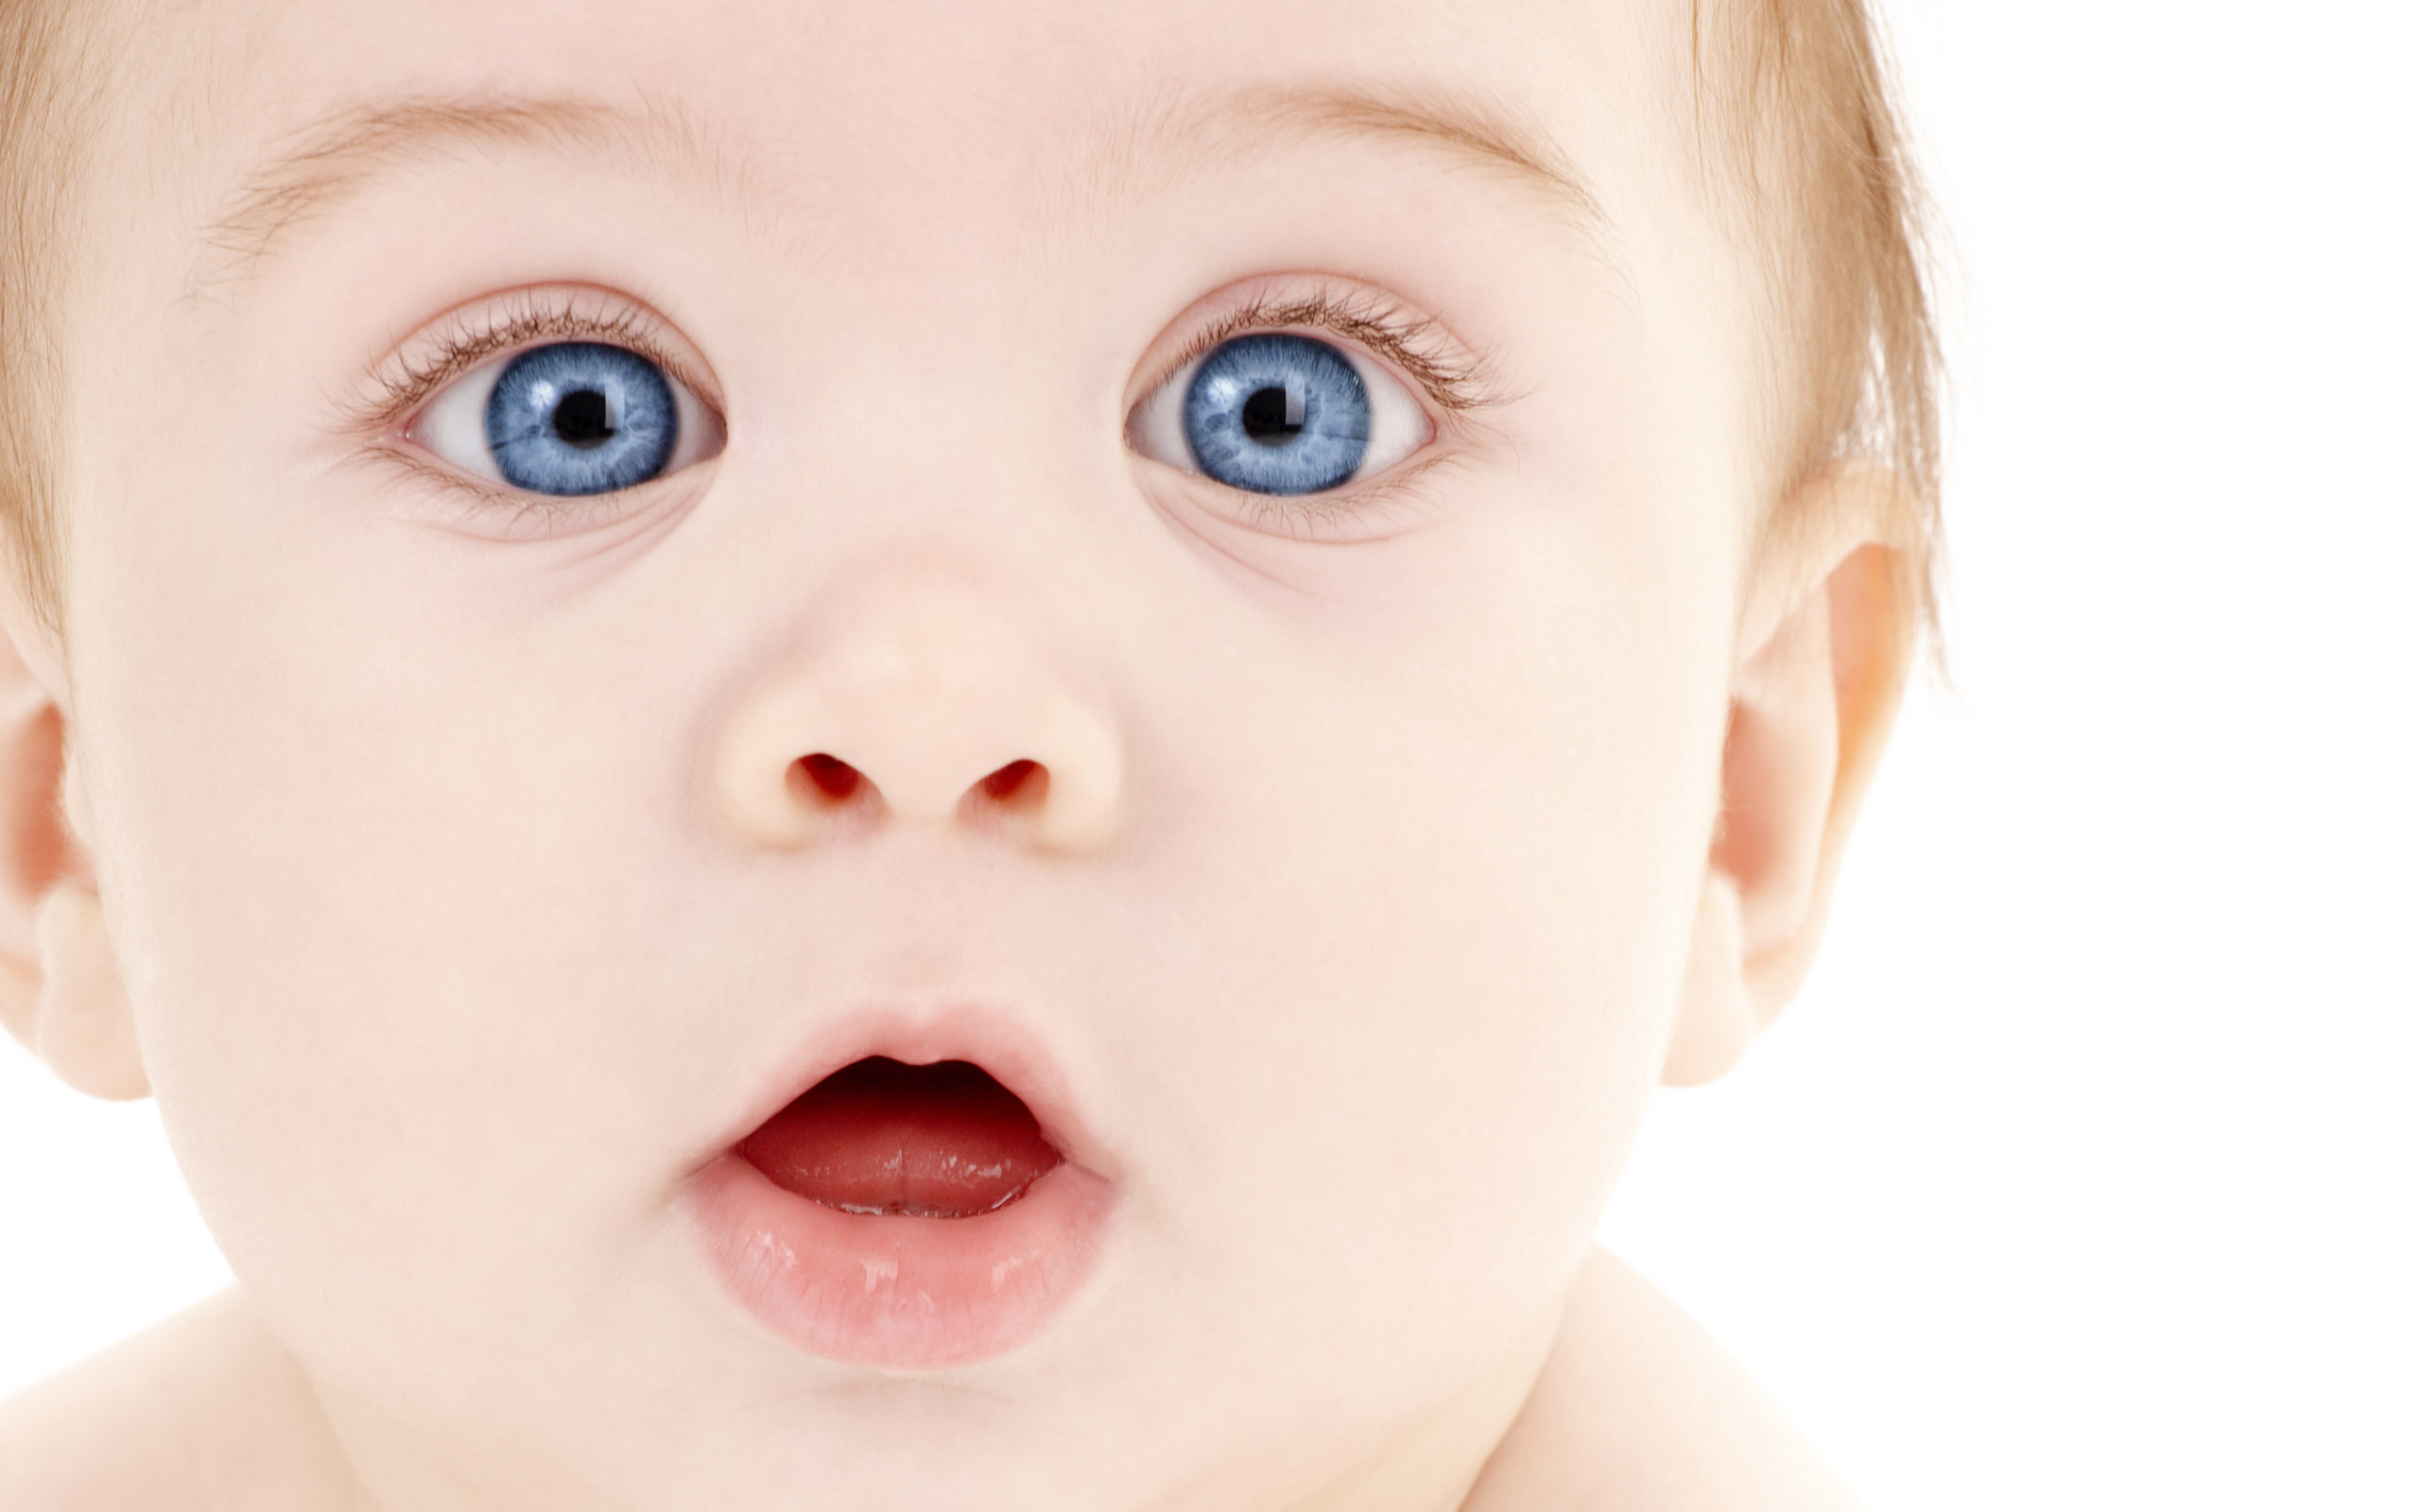
\includegraphics[height=\paperheight]{img/baby.jpg}} 
    \begin{frame}
        \begin{center}
            {\Huge \textbf{KNIFE THE BABY}}
        \end{center}
    \end{frame}
}

\begingroup
\setbeamercolor{background canvas}{bg=title}
\begin{frame}
    \begin{center}
        \vspace{1cm}
        {\Large\color{background} Maintenir son \textbf{\{code\}}}
    \end{center}
\end{frame}
\endgroup

\begin{frame}[fragile]
    \begin{columns}[c]
        \column{2.3in}
    \begin{center}{\large Field (champ)}\end{center}
        \begin{csharpcode*}{fontsize=\scriptsize}
public class Truc
{
    public int Attribut;
}
        \end{csharpcode*}
        \pause
        \begin{csharpcode*}{fontsize=\scriptsize}
public class ...
{
    public void MaFonction(...)
    {
        Truc machin = new Truc();

        Console.Write(Truc.Attribut);
    }
}
        \end{csharpcode*}
        \pause
        \column{2.2in}
        \begin{center}
            {\large Property (propriété)}\\
            \emph{\scriptsize Snippet VS : propfull}
        \end{center}
        \begin{csharpcode*}{fontsize=\scriptsize}
public class Truc
{
    // backing field
    private int _attribut;

    public int Attribut // propriété
    {
        get { return _attribut; }
        set { _attribut = value; }
    }
}
        \end{csharpcode*}
    \end{columns}
\end{frame}

\begin{frame}[fragile]
    \begin{center}{\large Validation}\end{center}
    \begin{csharpcode*}{fontsize=\scriptsize}
class Thermostat
{
    private int _temperature; // backing field

    public int Temperature // propriété
    {
        get { return _temperature }
        set
        {
            if(value >= 50)
                _temperature = 50;
            else
                _temperature = value;
        }
    }
}
    \end{csharpcode*}
\end{frame}

\begin{frame}[fragile]
    \begin{center}
        {\large Auto-propriété}\\
        \emph{\scriptsize Snippet VS : prop}
    \end{center}
    \begin{csharpcode}
public class Objet
{
    public int Attribut { get; set; };
}
    \end{csharpcode}
    \pause
    \begin{center}
        {\large Accès privé sur le \emph{set}}\\
        \emph{\scriptsize Snippet VS : propg}
    \end{center}
    \begin{csharpcode}
public class Objet
{
    public int Attribut { get; private set; };
}
    \end{csharpcode}
\end{frame}

\begin{frame}[fragile]
    \begin{center}{\large Interface}\end{center}
    \begin{csharpcode*}{fontsize=\scriptsize}
interface IBicycle
{
     string BrandName { get; set; }

     void ChangeSpeed(int newValue);

     void Brake();
}
    \end{csharpcode*}
    \pause
    \begin{csharpcode*}{fontsize=\scriptsize}
class BlueBicycle : IBicycle
{
    private string _brandName;

    public string BrandName
    {
        get { return _brandName }
        set { _brandName = lowerCase(value); }
    }
}
    \end{csharpcode*}
\end{frame}

\begin{frame}
    \begin{center}
        \vspace{1.1cm}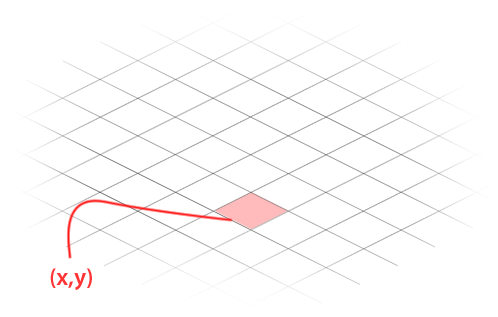
\includegraphics[scale=0.4]{img/map.png}
    \end{center}
\end{frame}

\begin{frame}<1-2>[label=unitbuilding,fragile]
\only<1>{\begin{center}\vspace{2.4cm}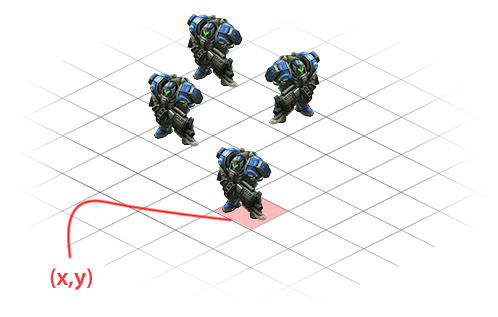
\includegraphics[scale=0.4]{img/unit.png}\end{center}}\pause
\begin{center}{\large Modélisation d'une unité \uncover<3->{et d'un bâtiment}}\end{center}
    \begin{columns}[c]
        \column{2.3in}
        \begin{csharpcode*}{fontsize=\tiny}
class Unit
{
    public Tuple<int,int> Position { get; set; }

    public int HealthPoints { get; set; }
    private int _maxHealthPoints;

    public int Speed { get; private set; }

    public int Dps { get; private set; }

    public void Move(Tuple<int,int> destination)
    {
        // Bouger
    }

    public void Die()
    {
        // Mourir
    }
}
        \end{csharpcode*}
        \pause
        \column{2.5in}
        \begin{csharpcode*}{fontsize=\tiny}
class Building
{
    public Tuple<int,int> Position { get; private set; }
    public Tuple<int,int> Size { get; private set; }

    public List<Unit> Units { get; set; }

    public int HealthPoints { get; set; }
    private int _maxHealthPoints;

    public void Die()
    {
        // Mourir
    }
}
        \end{csharpcode*}
    \end{columns}
\end{frame}

\begin{frame}
    \begin{center}
        \vspace{1.4cm}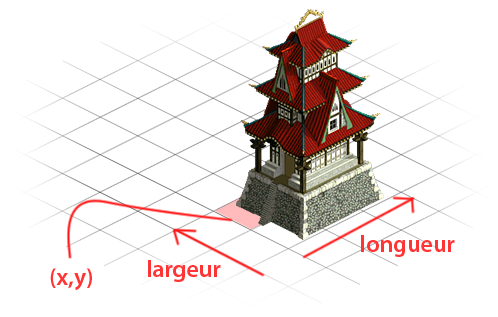
\includegraphics[scale=0.4]{img/building.png}
    \end{center}
\end{frame}

\againframe<3->{unitbuilding}

\begin{frame}[fragile]
    \begin{columns}[c]
        \column{2.3in}
        %\begin{center}{\large Classe Abstraite}\end{center}
        \begin{csharpcode*}{fontsize=\scriptsize}
abstract class GameItem
{
    public Tuple<int,int> Position
        { get; private set; }

    public int HealthPoints
        { get; set; }
    
    private int _maxHealthPoints;

    public abstract void Die();
}
        \end{csharpcode*}
        \pause
        \begin{csharpcode*}{fontsize=\scriptsize}
class Building : GameItem
{
    public Tuple<int,int> Size
        { get; private set; }

    public List<Unit> Units
        { get; set; }

    public override void Die()
    {
        // Mourir
    }
}
        \end{csharpcode*}
        \column{2.3in}
        \pause
        \begin{csharpcode*}{fontsize=\scriptsize}
class Unit : GameItem
{
    public int Speed
        { get; private set; }

    public int Dps
        { get; private set; }

    public void Move(
        Tuple<int,int> destination)
    {
        // Bouger
    }

    public override void Die()
    {
        // Mourir
    }
}
        \end{csharpcode*}
        \pause
        \begin{center}{\large Refactorisation !}\end{center}
    \end{columns}
\end{frame}

\begin{frame}[fragile]
    \begin{csharpcode}
class ...
{
    public void Fonction(...)
    {
        List<GameItem> gameItems = new List<GameItem>();

        gameItems.Add(new Unit());
        gameItems.Add(new Building());

        ...
    }
}
    \end{csharpcode}
\end{frame}

\begin{frame}[fragile]
    \begin{center}{\large Virtual methods}\end{center}
    \begin{csharpcode*}{fontsize=\scriptsize}
abstract class Truc
{
    public virtual void Fonction(int parameter)
    {
        // Faire quelque chose
    }
}
    \end{csharpcode*}
    \pause
    \begin{columns}
        \column{2.8in}
        \begin{csharpcode*}{fontsize=\scriptsize}
class Machin : Truc
{
    public override void Fonction(int parameter)
    {
        // Faire quelque chose d'autre

        base.Fonction(parameter);
    }
}
        \end{csharpcode*}
        \column{1.6in}
        \begin{csharpcode*}{fontsize=\scriptsize}
class Machin2 : Truc
{
}
        \end{csharpcode*}
    \end{columns}
\end{frame}

\begin{frame}
    \begin{center}
        {\large Architecture du code source}\\
        \vspace{0.2cm}
        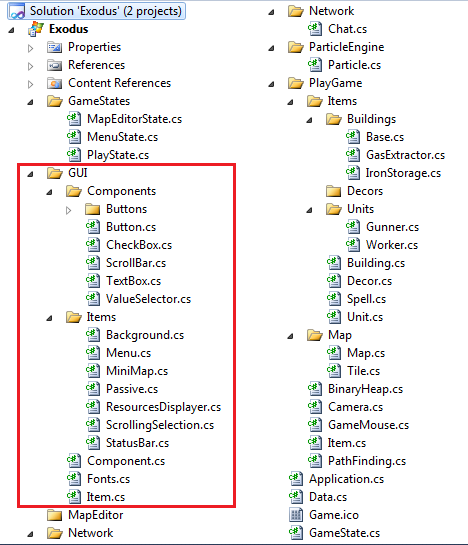
\includegraphics[scale=0.35]{img/archi.png}
    \end{center}
\end{frame}

{ % all template changes are local to this group.
    \setbeamertemplate{navigation symbols}{}
    \begin{frame}[plain]
        \begin{tikzpicture}[remember picture,overlay]
            \node[at=(current page.center)] {
                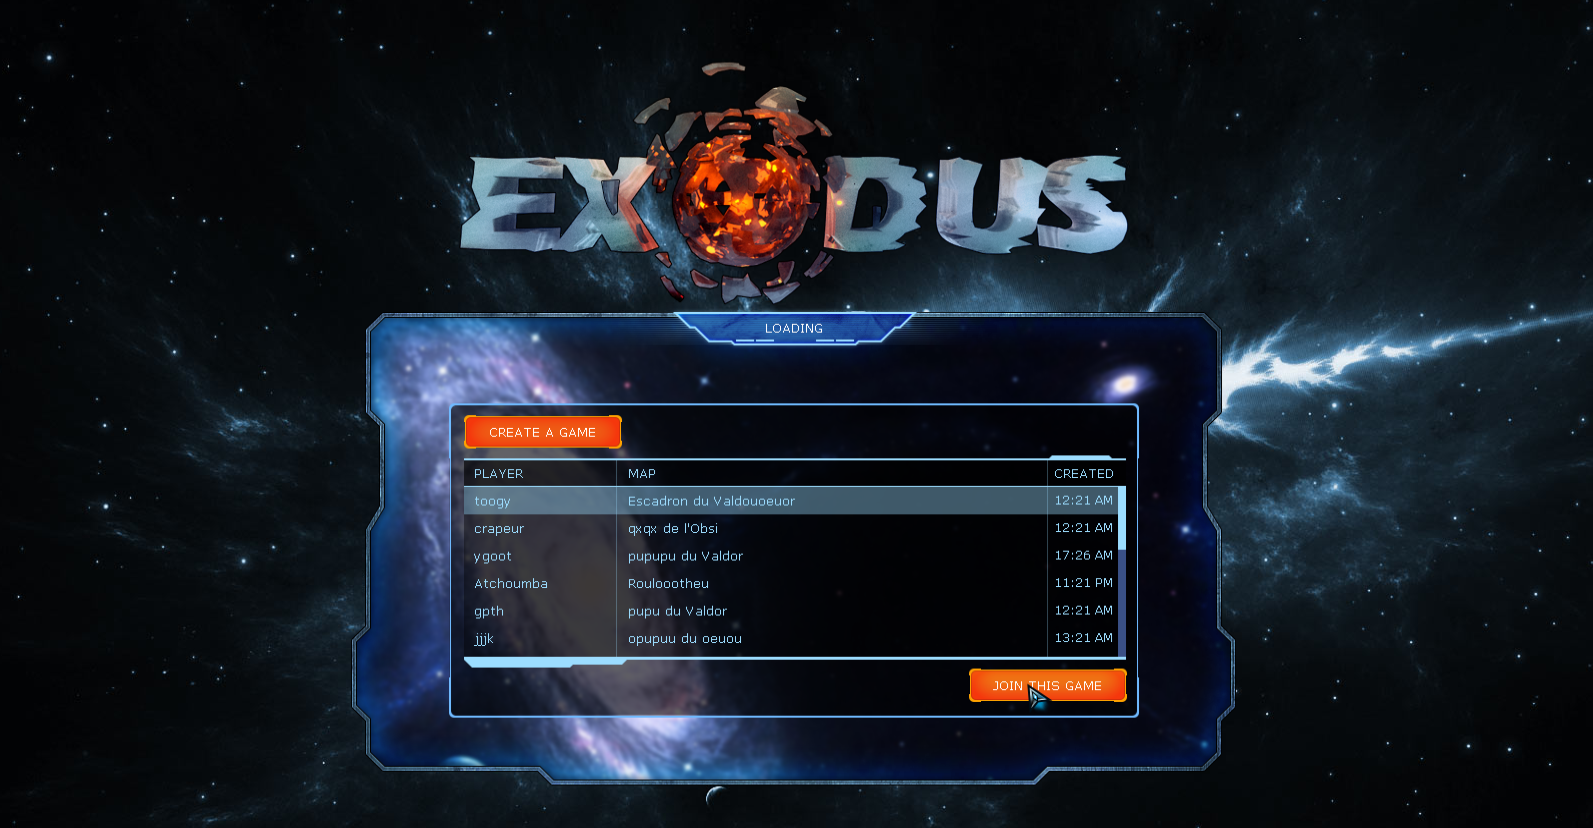
\includegraphics[height=\paperheight]{img/exodus-menu-ui.jpg}
            };
        \end{tikzpicture}
    \end{frame}
}

\begin{frame}
    \begin{center}
        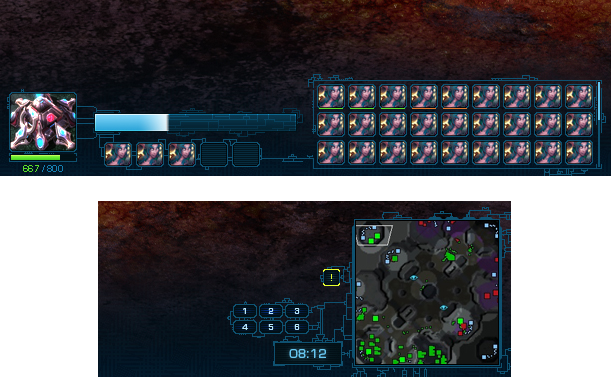
\includegraphics[scale=0.4]{img/exodus-ig-ui.png}
    \end{center}
\end{frame}

\begin{frame}
    \begin{center}
        \vspace{1cm}
        \includegraphics[scale=0.5]{img/gamestate.eps}
    \end{center}
\end{frame}

\section{Git et le versioning}

\begingroup
\setbeamercolor{background canvas}{bg=foreground}
\begin{frame}
    \begin{center}
        \vspace{1cm}
        {\Large\color{background} \textbf{2. Git} et le versioning}
    \end{center}
\end{frame}
\endgroup

\section{\LaTeX}

\begingroup
\setbeamercolor{background canvas}{bg=latexblue}
\begin{frame}
    \begin{center}
        \vspace{1cm}
        {\Huge\color{background} \textbf{3.} {\fontencoding{T1}\fontfamily{anttlc}\fontseries{m}\fontshape{n}\selectfont\LaTeX}}
    \end{center}
\end{frame}
\endgroup

\section{DirectX et C\#}

\begingroup
\setbeamercolor{background canvas}{bg=title}
\begin{frame}
    \begin{center}
        \vspace{1cm}
        {\Large\color{background} \textbf{4.} DirectX et C\#}
    \end{center}
\end{frame}
\endgroup

\begin{frame}
    \begin{center}
        \includegraphics[scale=0.35]{img/arys1.eps}
    \end{center}
\end{frame}

\begin{frame}
    \begin{center}
        \includegraphics[scale=0.35]{img/arys2.eps}
    \end{center}
\end{frame}

\begin{frame}
    \begin{center}
        \includegraphics[scale=0.35]{img/arys3.eps}
    \end{center}
\end{frame}

\section{Introduction à XNA}

\begin{frame}
    \begin{center}
        \vspace{1cm}

        {\Large \textbf{4.} Introduction à XNA} \\

        \vspace{0.5cm}

        
\includegraphics[scale=0.65]{img/rd.png}
    \end{center}
\end{frame}

\begin{frame}
    \vspace{1cm}
    \begin{center}
        \includegraphics[scale=0.44]{img/xna-axis.eps}
    \end{center}
\end{frame}

\begin{frame}[fragile]
    \begin{csharpcode*}{fontsize=\scriptsize}
        public class Game : Microsoft.Xna.Framework.Game
        {
            readonly GraphicsDeviceManager _graphics;
            SpriteBatch _spriteBatch;

            public Game() { ... }

            protected override void Initialize() { ... }

            protected override void LoadContent() { ... }

            protected override void UnloadContent() { ... }

            protected override void Update(GameTime gameTime)
            {
                // Logique du jeu
            }

            protected override void Draw(GameTime gameTime)
            {
                // Affichage du jeu
            }
        }
    \end{csharpcode*}
\end{frame}

\begin{frame}
    \begin{center}
        \vspace{1cm}
        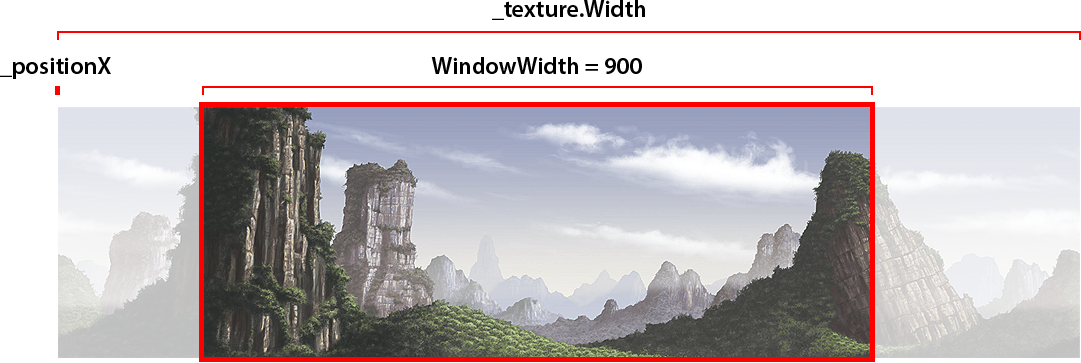
\includegraphics[scale=0.26]{img/bg1.png}
    \end{center}
\end{frame}

\begin{frame}
    \begin{center}
        \vspace{1cm} 
        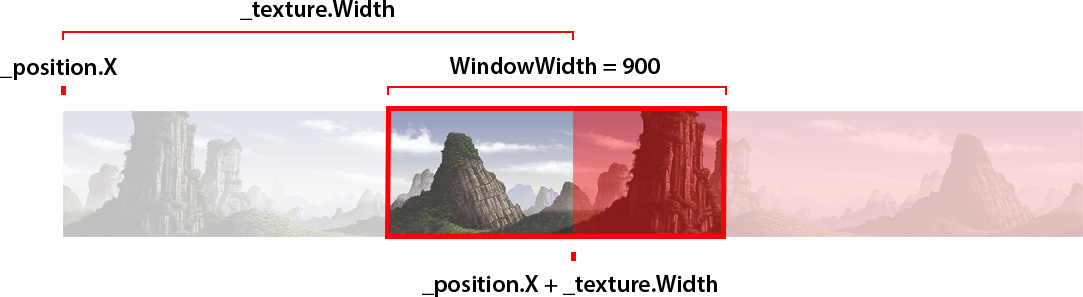
\includegraphics[scale=0.26]{img/bg2.png}
    \end{center}
\end{frame}

\section{TP Git \& XNA par équipe}

\begingroup
\setbeamercolor{background canvas}{bg=foreground}
\begin{frame}
    \begin{center}
        \vspace{1cm}
        {\Large\color{background} \textbf{TP} Git/XNA par équipe}
    \end{center}
\end{frame}
\endgroup

\end{document}
